
\chapter{Methodology}
To answer \textbf{RQ1}, we develop, train, and evaluate a model conditioned with inner metric weight. \textbf{RQ2} and \textbf{RQ3} are answered using a user study that collects metrics on player interactions with the music alongside survey responses. 

\section{The Model}
Sections \ref{section:non_neural_generation} and \ref{section:deep_learning_generation} discussed the potential approaches to music generation with particular attention to state-of-the-art approaches using deep learning. The developed model will be a transformer due to its ability to effectively model various sequences and its potential to incorporate additional controls. We will use a symbolic representation of music (as discussed in section \ref{section:symbolic_audio}) due to its lightweight datasets and the ability to make changes to and incorporate the output into a music production environment, enabling a cooperative co-composition process as opposed to replacing the composer. More specifically, we will use a representation similar to REMI+ (see section \ref{section:symbolic_tok}), which extends the standard MIDI events with tokens indicating forms, such as meter, bar lines, and note-duration. This representation is compounded using byte pair encoding (see section \ref{section:symbolic_tok}) to decrease the sequence length and improve the capability and efficiency of the model. For adding control (section \ref{section:addingcontrol}) we focus on methods that don't require full training, specifically parameter-efficient fine-tuning. This is more cost-effective and environmentally friendly. 
We will use the Lakh Midi Dataset \cite{Raffel_2016}, a widely used open-source and licensed dataset for symbolic music generation. This will help us avoid ethical pitfalls around privacy and copyright. (section \ref{section:ethical}). Finally, we are not attempting to add control by training custom large foundation models, rather we are using parameter-efficient fine-tuning or guidance (section \ref{section:addingcontrol}) to add control. As a result, we are using only a fraction of the model parameters, with substantially less need for data, computation, and energy. All relevant code, including code for training, configuration, and data preparation will be made available online alongside the model weights. Finally, we use and extend an open-source model MusicLang in collaboration with its maintainers. If successful these extensions will contribute to the MusicLang project and be widely available in a well-documented and continuously maintained ecosystem, with integrations into mainstream music production and composition software. 

\section{Developing the Model}

\subsection{Preliminary Experiments - proof of concept}
The current methods of adding musical control to an existing model are poorly systematized and rarely compared to each other. While this thesis does not aim to provide a systemic comparison and experimental evaluation of different control methods, some preliminary experiments are necessary to establish the best course of action. We use BassCraft, a smaller model, and start by controlling for note density (the number of notes in a bar). Note density is more easily calculated, tokenized, and verified than inner metric weight.  

\subsubsection{BassCraft -  a tiny transformer model}
To avoid wasting valuable computing resources and energy, we perform the preliminary experiments on a smaller model: Basscraft. BassCraft is a small transformer model based on  GPT2 \cite{Radford_Wu_Child_Luan_gpt2_2019}. It has an embedding size of 256, 4 attention heads, four hidden transformer layers, and 7 million trainable parameters. In contrast, the target LLAMA 2-based model MusicLang has over 100 million trainable parameters. Basscraft generates a bassline to a provided piece of music and is trained on the lakh-midi dataset \cite{Raffel_2016}. For training, songs with bass lines are selected (based on the presence of particular MIDI-instrument channels). The tracks are divided into snippets between 1 and 16 bars long. The bass lines are separated from the remaining track and matched as potential output. 

\begin{figure}[H]
    \centering
    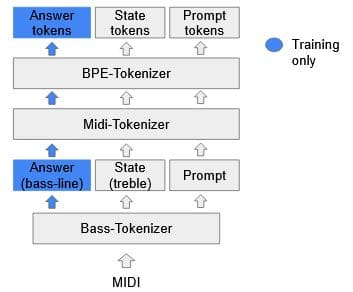
\includegraphics[width=0.5\textwidth]{IMAGES/Preprocessing1.jpg} 
    \caption{Preprocessing and tokenization of the original basscraft model}
    \label{fig:preprocessing1}
\end{figure}

\subsubsection{Fine-Tuning 1 - Vocabulary Expansion}

Vocabulary expansion is the process of adding new vocabulary to a transformer model. MusicLang achieves its extraordinary controllability similarly to FIGARO \cite{Rütte_figaro_2023} using control tokens that summarize features of the music that go beyond simply representing MIDI events. In vocabulary extension, it is critical to ensure that additional tokens do not overwrite or otherwise collide with the existing training. Otherwise, the benefits of using a pre-trained model disappear. Since we use a BPE tokenizer, it is difficult to add new tokens, as it would require retraining the BPE tokenizer, which will transform the embedding layer, making the entire model unusable. Instead, we investigate whether there are unused tokens and reassign them to our new control tokens. These new tokens are not included in any compound tokens generated by the BPE process, which increases the sequence length.

\begin{figure}[H]
    \centering
    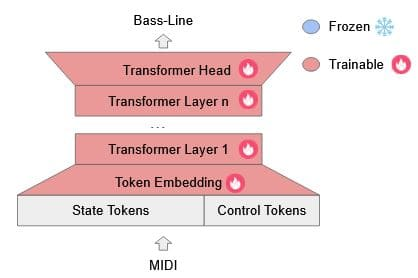
\includegraphics[width=0.5\textwidth]{IMAGES/full_ft.jpg}
    \caption{Vocabulary transfer with full fine tuning}
    \label{fig:vocabtrans1}
\end{figure}

\begin{figure}[H]
    \centering
    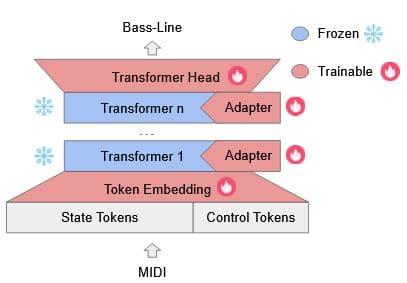
\includegraphics[width=0.5\textwidth]{IMAGES/vocab_lora_ft.jpg} 
    \caption{Vocabulary transfer with parameter efficient fine tuning}
    \label{fig:vocabtrans2}
\end{figure}

\subsubsection{Fine-Tuning 2 - Integrating of control tokens} 

This approach differs from vocabulary expansion because it processes the control tokens as a parallel stream. This is similar to the approach used in Coco-Mulla \cite{Lin_cocomulla_2024}. After passing through a trainable positional embedding, the parallel stream of control tokens is inserted into the model at a layer $c$. The benefit of this method is that it doesn't require editing the model's vocabulary. 
 
\begin{figure}[H]
    \centering
    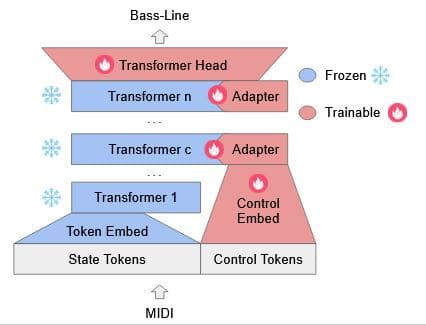
\includegraphics[width=0.5\textwidth]{IMAGES/ControlTokensLora.jpg} 
    \caption{Integration of control tokens with parameter efficient fine tuning}
    \label{fig:controltok}
\end{figure}

\subsubsection{Post-Hoc Guidance and other improvements}

SMITIN\cite{Koo_Wichern_Germain_SMITIN_2024} uses post-hoc guidance on a trained model to influence the generation process without retraining the model. This type of sampling-based guidance has been very successful in diffusion models. In transformers, however, it produces mixed results \cite{language_guide_rutte_2024}.  Additionally, this may be difficult to implement and transfer to inner metric weight. Both SMITIN and Rütte\cite{language_guide_rutte_2024} only use one-dimensional variables that indicate the probability of a concept being present or not. 

\begin{figure}[H]
    \centering
    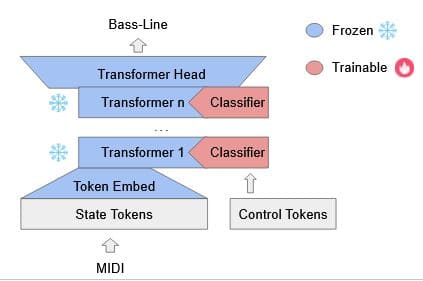
\includegraphics[width=0.5\textwidth]{IMAGES/adhoccontrol.jpg} 
    \caption{Integration of control using inference time interference}
    \label{fig:adhoccontrol}
\end{figure}

If these experiments are unsuccessful, we can follow the approach of \cite{Shu_Xu_Musebarcontrol_2024} and try additional training using auxiliary tasks or use a modified (counterfactual) loss function. 

\subsection{Using inner metric weight as controllable feature}
Inner metric analysis (IMA) creates metric weight profiles we use as guiding features passed to the model bar by bar, which allows us to induce shifts in metric weight in the output. 
For this, we use the globally smallest available note grid of the lakh-midi dataset $g_min$. These distributions are normalized and provided to the model as vectors of length $g_{min}$.
The model then learns embeddings of the distribution alongside positional embeddings \cite{Lin_cocomulla_2024}. These embeddings are then incorporated into the model. For inference, the user can provide a reference track from which the inner metric profile is extracted and passed to the model. 
\begin{figure}[H]
    \centering
    \begin{subfigure}{0.45\textwidth}
        \centering
        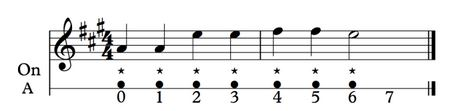
\includegraphics[width=\linewidth]{IMAGES/IMA1.JPG}
        \caption{Single local meter and its pulses (A) from the melody "Twinkle, Twinkle Little Star"}
        \label{fig:ima1}
    \end{subfigure}
    \begin{subfigure}{0.45\textwidth}
        \centering
        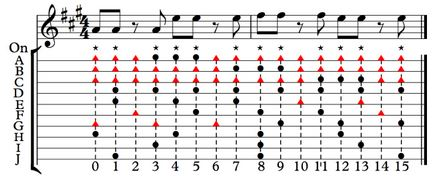
\includegraphics[width=\linewidth]{IMAGES/IMA2.JPG}
        \caption{10 local meters and their pulses produced by IMA of a syncopated variation of "Twinkle, Twinkle Little Star"}
        \label{fig:ima2}
    \end{subfigure}
    
    \vspace{0.5cm} % Adjust spacing between rows

    \begin{subfigure}{0.45\textwidth}
        \centering
        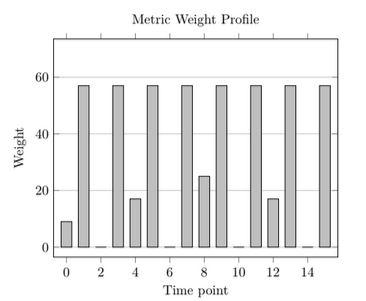
\includegraphics[width=\linewidth]{IMAGES/IMA3.JPG}
        \caption{Metric weight profile of syncopated "Twinkle, Twinkle Little Star"}
        \label{fig:ima3}
    \end{subfigure}
    \begin{subfigure}{0.45\textwidth}
        \centering
        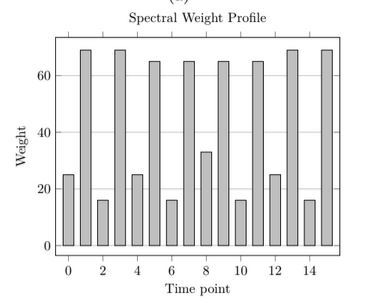
\includegraphics[width=\linewidth]{IMAGES/IMA4.JPG}
        \caption{Spectral weight profile of syncopated "Twinkle, Twinkle Little Star"}
        \label{fig:ima4}
    \end{subfigure}

    \caption{Visualisation of metric weight analysis \cite{Bemman2024}}
    \label{fig:ima_all}
\end{figure}

\subsection{MusicLang - The foundation Model}
To answer RQ1, we need to extend a music generator with control for inner metric weight. After concluding the preliminary experiments and identifying a promising set of methods of adding control and encoding inner metric weight, we will proceed with the larger MusicGen model. 
MusicLang's core model is a transformer based on LLAMA 2 trained on the Lakh Midi Dataset\cite{Raffel_2016}. It can generate relatively long multi-track instrumental pieces (1-3 minutes) with control for chord progression, instrumentation, and range. Additionally, it can create interpolations and continuations of a user-provided piece. It is trained on an extended vocabulary of tokens similar to REMI\footnote{https://musiclang.github.io/tokenizer/} with additional tokens detailing the harmonic structure and voice characteristics such as instrumentation or range (see figure \ref{fig:musiclangtok}). This base vocabulary is extended using a BPE tokenizer. 

\begin{figure}[H]
    \centering
    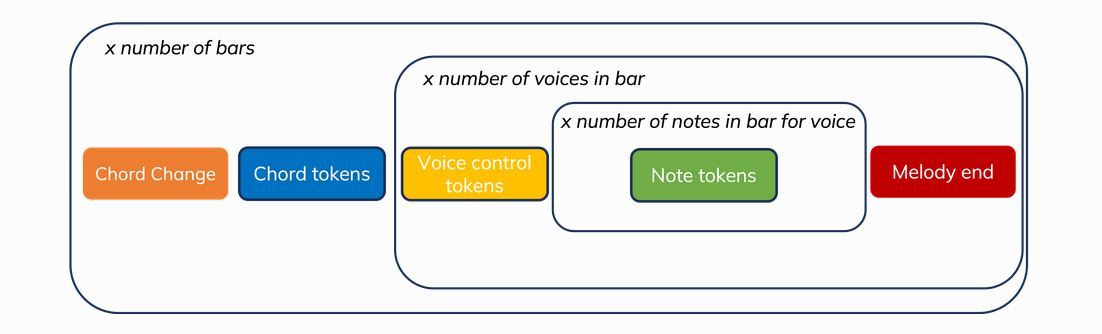
\includegraphics[width=0.5\textwidth]{IMAGES/MusicLang.JPG} 
    \caption{MusicLang tokenisation on a high level}
    \label{fig:musiclangtok}
\end{figure}

\subsection{Evaluating Control-Effectivness}
As discussed in section \ref{section:evaluation}, calculating whether or not the control is effective depends on the controlled feature but can happen automatically. 
The first set of experiments targets note density: If note density is a categorical variable such as low, medium, or high, the error is calculated similarly to a multilabel classifier. The predicted label is the note density of the generated music, and the ground-truth label is the note density given in the prompt on a bar-by-bar level. 
The metrics include accuracy, precision, recall, and F1 scores. 
If note density is continuous (the number of notes per bar), then the error would be calculated as mean square error: 
\begin{equation}
 error_{continuous} = \sqrt{\frac{1}{n}\sum_{j=1}^{n}(y_{generated}-y_{prompt})}
\end{equation}
Inner metric weight analysis generates metric weight profiles, which we use as a guidance mechanism. Following the approach by \cite{Bemman2024}, we can compare the generated and the target rhythmic weight profiles using chi-squared distance.
Given target distribution $T$ and generated distribution $G$, the distance is given by 
\begin{equation}
D=\sum_{i=0}^{n-1}(\frac{(T_i-G_i)^2}{T_i+G_i})
\end{equation}

\section{User Study}
\textbf{RQ2} and \textbf{RQ3} are evaluated through a user study. The goal is to recruit $n=20$ participants to complete a test of interactability and a survey comparatively evaluating the generated music. 
\subsection{Interactive Study}
The interactive study aims to evaluate the fitness of the controlled generated music from an MACT perspective. Specifically, in the MACT protocol used by Chalkiadakis \cite{Chalkiadakis_2022}, the patient is supposed to listen to changes in the music and change their playing. In our simplified interactive sessions the player is asked to hit a button whenever they hear a change in the music. The button presses are registered alongside the starting time, tempo, and registered changing points (determined from the prompt). Finally, the timing of the button presses and registered changes are correlated with each other. A high correlation indicates that the participants noticed the changes. 

\subsection{Survey}
The survey will compare the listening experience of different symbolic generative models, including our model, FIGARO \cite{Rütte_figaro_2023} and Polyfussion \cite{Min_Jiang_Xia_Zhao_polyffusion_2023} as well as the improved rule-based generator of "Last Minute Gig" \cite{Chalkiadakis_2022}\cite{Schlette_2022}. The questionnaire asks the participants to rate coherence richness arrangement and consistency on a selection of tracks by the different models. 
The questionnaire also includes questions on demographic information such as gender, age, and educational background, but also musical experience.

\section{Thesis Timeline}

\begin{figure}[H]
    \centering
    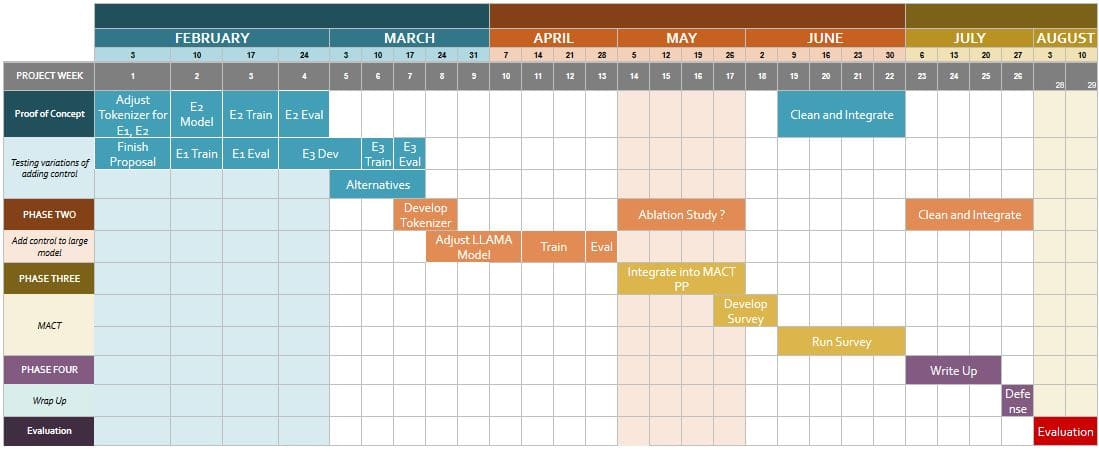
\includegraphics[width=1\textwidth]{IMAGES/project_plan.jpg} 
    \caption{Thesis project plan}
    \label{fig:projectplan}
\end{figure}


